\chapter{Pola Perilaku 2}



\section{Pola Perilaku Lanjutan}

Pola desain perilaku lanjutan merupakan kelanjutan dari pendekatan pemrograman berorientasi objek yang berfokus pada bagaimana objek saling berinteraksi dan bagaimana alur kendali dibentuk di dalam sistem perangkat lunak yang kompleks. Bab ini membahas empat pola penting—\textit{Mediator}, \textit{State}, \textit{Chain of Responsibility}, dan \textit{Template Method}—yang dirancang untuk menyederhanakan komunikasi antar objek, mengatur transisi keadaan secara dinamis, mendistribusikan tanggung jawab secara berantai, dan mendefinisikan kerangka algoritma dengan fleksibilitas pada langkah-langkah tertentu. Pemahaman terhadap pola-pola ini memungkinkan perancang sistem untuk menciptakan arsitektur perangkat lunak yang lebih modular, dapat diperluas, dan mudah dipelihara.



\section{Mediator}
\subsection{Tujuan dan Konteks Penggunaan}

Pola \textit{Mediator} adalah pola desain perilaku yang bertujuan untuk mengurangi kompleksitas komunikasi antar objek dengan memperkenalkan satu objek pengatur — disebut \texttt{Mediator} — yang bertanggung jawab untuk mengoordinasikan interaksi antar objek (komponen). Pola ini membantu menghindari hubungan banyak-ke-banyak antar objek, yang dapat menyebabkan sistem menjadi sulit dipelihara, diperluas, dan diuji.

Alih-alih objek saling merujuk dan saling berkomunikasi secara langsung, semua komunikasi dilakukan melalui mediator. Dengan demikian, objek menjadi lebih terpisah dan tidak mengetahui detail objek lain, hanya bergantung pada mediator untuk berinteraksi.

Pola \textit{Mediator} sangat sesuai digunakan ketika:
\begin{itemize}
	\item Banyak objek berinteraksi secara kompleks dan saling bergantung.
	\item Ingin mengurangi keterikatan antar komponen agar lebih mudah diuji dan diubah secara independen.
	\item Ingin memusatkan aturan koordinasi dan interaksi dalam satu tempat agar lebih terkelola.
	\item Sistem UI atau komponen form interaktif yang saling memengaruhi (misalnya: input A mengubah validitas input B dan C).
\end{itemize}

Struktur utama pola \textit{Mediator} melibatkan:
\begin{itemize}
	\item \textbf{Mediator (Interface):} Mendefinisikan kontrak komunikasi antar komponen.
	\item \textbf{ConcreteMediator:} Implementasi mediator yang mengelola interaksi antar objek konkret.
	\item \textbf{Colleague:} Objek partisipan yang merujuk ke mediator untuk semua interaksi, bukan ke objek lain secara langsung.
\end{itemize}

Dengan memanfaatkan pola ini, sistem dapat mencapai arsitektur yang lebih modular dan memudahkan perubahan perilaku antar komponen tanpa perlu mengubah logika internal masing-masing komponen secara langsung.

\subsection{Contoh Kasus Penggunaan}

Pola \textit{Mediator} banyak digunakan dalam skenario di mana terdapat interaksi kompleks antar banyak komponen, dan diperlukan pemusatan logika komunikasi agar sistem lebih mudah dipelihara. Berikut beberapa contoh kasus nyata penerapannya:

\textbf{1. Formulir Interaktif pada Antarmuka Pengguna (UI)} \\
Dalam sebuah form pendaftaran, input seperti pilihan jenis akun dapat memengaruhi visibilitas atau status aktif input lainnya (misalnya, kolom nomor perusahaan hanya muncul jika pengguna memilih “akun bisnis”). Daripada setiap input saling mengetahui dan mengatur satu sama lain, sebuah \texttt{FormMediator} bisa digunakan untuk mengatur semua logika ini secara terpusat.

\textbf{2. Dialog Komponen dalam GUI Framework} \\
Pada jendela dialog yang terdiri dari tombol, kolom teks, dan daftar pilihan, masing-masing komponen tidak saling mengenal. Ketika suatu tombol ditekan, mediator (misalnya \texttt{DialogBoxMediator}) menentukan komponen lain mana yang perlu diperbarui atau dikunci, sesuai aturan logika dialog tersebut.

\textbf{3. Chat Room atau Message Hub} \\
Dalam sistem chat, alih-alih user mengirimkan pesan langsung ke user lain, setiap pesan dikirim melalui objek \texttt{ChatMediator}. Mediator ini bertanggung jawab untuk menyampaikan pesan ke peserta yang sesuai, mencatat histori, atau melakukan validasi konten pesan.

\textbf{4. Komunikasi antar Komponen Pesawat (Avionik)} \\
Dalam sistem avionik modern, berbagai subsistem seperti navigasi, kontrol mesin, autopilot, dan sensor cuaca saling terhubung. Menggunakan mediator, komunikasi dan koordinasi antar subsistem dilakukan secara terpusat untuk menghindari jaringan komunikasi yang terlalu rumit dan berisiko tinggi.

\textbf{5. Sistem Game: Karakter atau Objek Interaktif} \\
Dalam game strategi, berbagai unit atau karakter mungkin berinteraksi berdasarkan kondisi lingkungan atau status unit lain. Mediator seperti \texttt{GameMediator} dapat mengatur efek global, mengkoordinasi interaksi antar unit, atau memicu event berdasarkan kondisi kompleks antar elemen game.

\textbf{6. Manajemen Komponen dalam Sistem IoT atau Smart Home} \\
Berbagai perangkat seperti sensor gerak, lampu, kamera, dan alarm bisa diatur melalui \texttt{SmartHomeMediator}. Ketika sensor mendeteksi gerakan, mediator memutuskan apakah harus menyalakan lampu, memulai perekaman kamera, atau mengirim notifikasi ke pemilik.

Melalui pola ini, sistem menjadi lebih terstruktur dan interaksi antar objek tidak mengakibatkan peningkatan kompleksitas yang tidak terkendali, sehingga mudah diperluas dan dipelihara.

\subsection{Kelebihan dan Kekurangan}

Pola \textit{Mediator} dirancang untuk mereduksi kompleksitas komunikasi antar objek dengan memindahkan interaksi langsung antar objek ke dalam satu entitas pusat. Pendekatan ini sangat bermanfaat untuk sistem yang melibatkan banyak komponen dengan interaksi saling terkait. Namun, seperti semua pola desain, terdapat kelebihan dan kekurangan yang perlu dipertimbangkan sebelum menerapkannya.

\textbf{Kelebihan:}
\begin{itemize}
	\item \textbf{Mengurangi coupling antar objek:} Objek tidak lagi saling bergantung secara langsung, karena hanya berkomunikasi melalui mediator. Hal ini mendukung prinsip \textit{loose coupling} dan mempermudah penggantian atau pengujian komponen secara terpisah.
	
	\item \textbf{Meningkatkan keterbacaan dan pemeliharaan:} Dengan memusatkan logika komunikasi, pola ini membuat kode lebih mudah dibaca dan dikelola. Perubahan dalam pola interaksi cukup dilakukan pada mediator, tanpa harus mengubah setiap komponen.
	
	\item \textbf{Memfasilitasi koordinasi kompleks:} Pola ini sangat cocok ketika terdapat banyak komponen yang perlu saling berinteraksi berdasarkan kondisi tertentu. Mediator dapat mengimplementasikan logika koordinasi ini secara eksplisit dan terorganisasi.
	
	\item \textbf{Memisahkan tanggung jawab:} Komponen tidak lagi memuat logika komunikasi, sehingga masing-masing dapat fokus pada tugas utamanya (misalnya, menangani input atau menampilkan data).
	
	\item \textbf{Mendukung pengujian modular:} Karena mediator mengisolasi interaksi, komponen individual dapat diuji secara terpisah menggunakan mediator palsu (mock) tanpa melibatkan seluruh sistem.
\end{itemize}

\textbf{Kekurangan:}
\begin{itemize}
	\item \textbf{Mediator bisa menjadi terlalu kompleks:} Saat jumlah interaksi dan aturan bertambah, mediator bisa tumbuh menjadi kelas raksasa (\textit{god object}) yang sulit dipelihara dan diuji.
	
	\item \textbf{Sulit dilacak dalam sistem besar:} Logika interaksi yang tersentralisasi di mediator dapat menyulitkan pemahaman aliran kontrol jika tidak diberi dokumentasi atau struktur yang baik.
	
	\item \textbf{Overhead tambahan untuk sistem sederhana:} Pada sistem dengan interaksi yang sangat sedikit atau statis, penggunaan mediator justru menambah lapisan abstraksi yang tidak diperlukan.
	
	\item \textbf{Ketergantungan pada mediator tunggal:} Semua komunikasi bergantung pada mediator, sehingga jika terjadi kesalahan atau perubahan besar pada mediator, dampaknya bisa luas ke seluruh sistem.
	
	\item \textbf{Potensi duplikasi jika ada banyak mediator:} Jika sistem terdiri dari banyak kelompok objek dengan mediator masing-masing, bisa terjadi pengulangan logika yang serupa di banyak tempat.
\end{itemize}

Secara keseluruhan, pola \textit{Mediator} ideal digunakan untuk mengelola interaksi antar banyak objek yang dinamis dan kompleks. Namun, penting untuk menjaga mediator tetap modular, terstruktur, dan tidak menjadi pusat dari terlalu banyak logika bisnis.



\subsection{Implementasi dalam Java}

Implementasi pola \textit{Mediator} dalam Java dilakukan dengan cara mendefinisikan antarmuka \texttt{Mediator} yang bertugas mengatur komunikasi antar objek, serta antarmuka atau kelas \texttt{Colleague} sebagai komponen yang berinteraksi melalui mediator. Setiap \texttt{Colleague} tidak saling berkomunikasi langsung, melainkan melalui objek mediator yang telah disuntikkan (injected) ke dalamnya.

Struktur implementasi umumnya terdiri dari:
\begin{itemize}
	\item \textbf{Mediator (Interface):} Mendefinisikan kontrak umum yang mengatur interaksi antar objek (colleague).
	\item \textbf{ConcreteMediator:} Implementasi spesifik dari \texttt{Mediator} yang mengetahui dan mengatur seluruh \texttt{Colleague}.
	\item \textbf{Colleague (Interface/Kelas Abstrak):} Komponen yang berinteraksi melalui mediator. Biasanya menyimpan referensi ke mediator.
	\item \textbf{ConcreteColleague:} Objek spesifik yang tidak langsung berkomunikasi dengan kolega lain, melainkan menggunakan mediator.
\end{itemize}

Contoh berikut mengilustrasikan pola \textit{Mediator} pada sistem dialog UI yang terdiri dari dua komponen: \texttt{Button} dan \texttt{TextBox}. Interaksi antara keduanya dikendalikan oleh objek mediator (Gambar~\ref{fig:mediator}).


\begin{figure}[h]
	\centering
	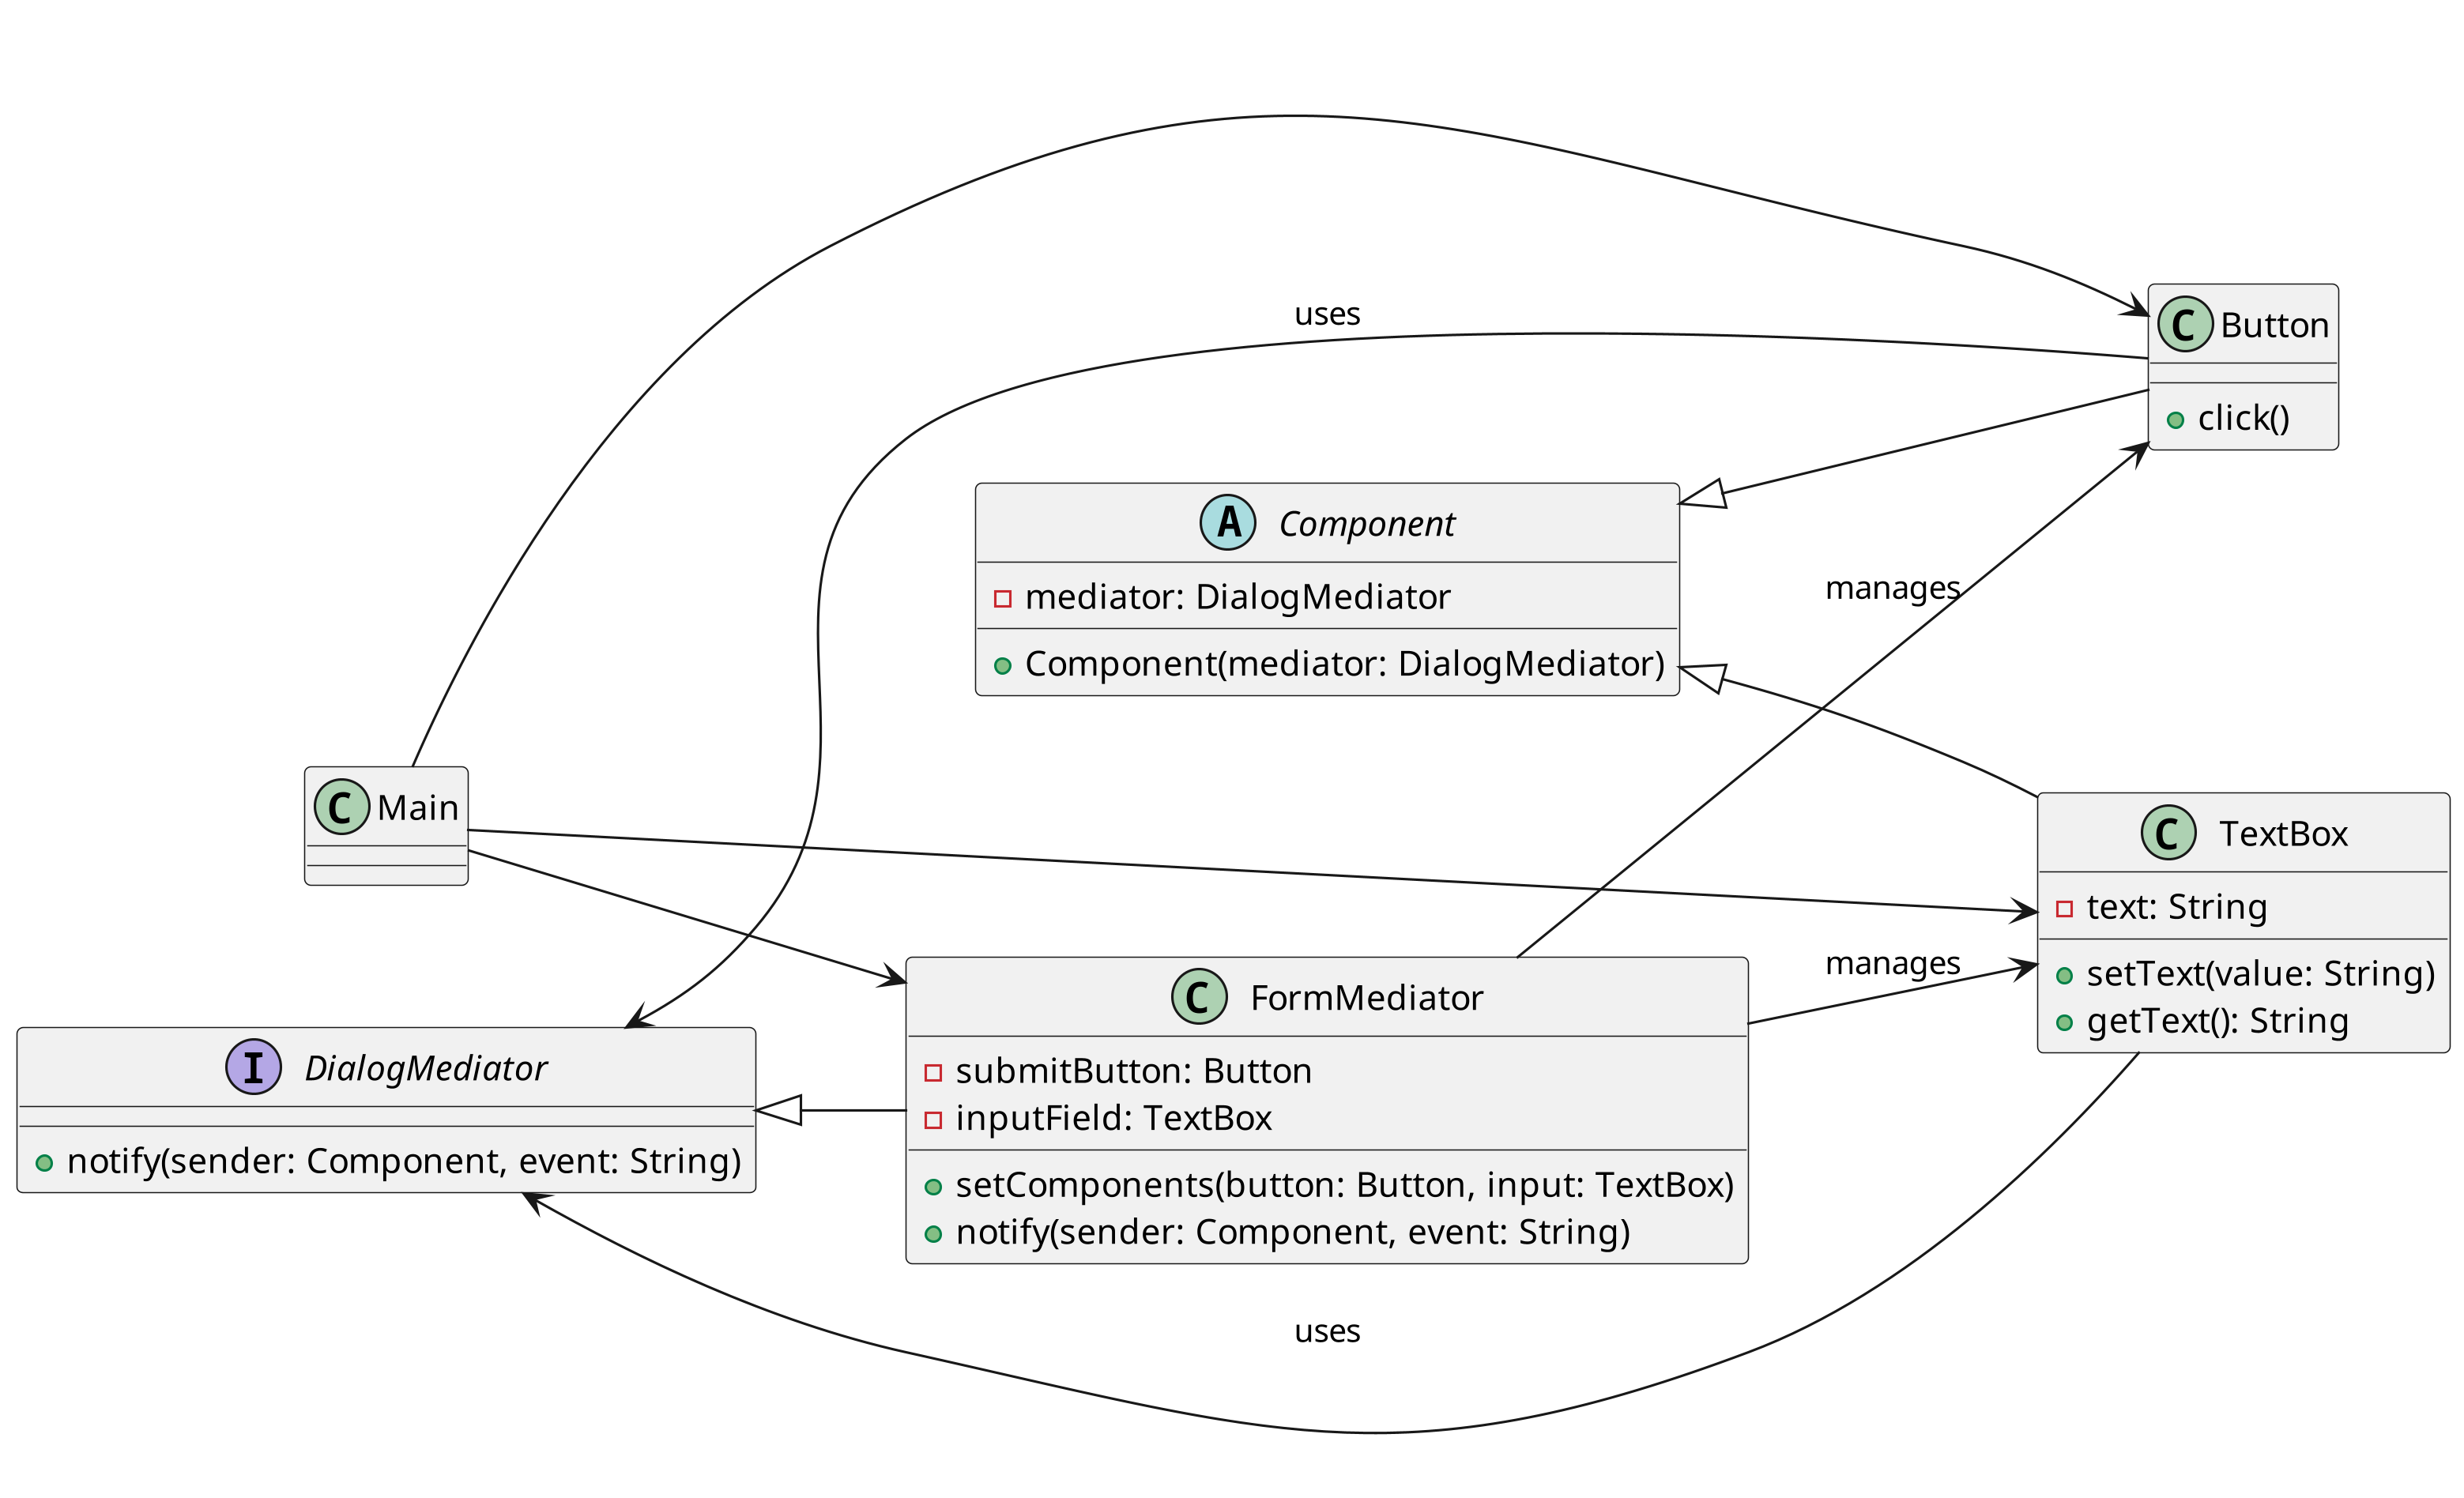
\includegraphics[width=\textwidth]{../figures/out/mediator.png}
	\caption{Struktur Pola Mediator}
	\label{fig:mediator}
\end{figure}


\begin{lstlisting}[style=JavaStyle, caption={Antarmuka Mediator}]
	public interface DialogMediator {
		void notify(Component sender, String event);
	}
\end{lstlisting}

\begin{lstlisting}[style=JavaStyle, caption={Kelas Komponen Umum}]
	public abstract class Component {
		protected DialogMediator mediator;
		
		public Component(DialogMediator mediator) {
			this.mediator = mediator;
		}
	}
\end{lstlisting}

\begin{lstlisting}[style=JavaStyle, caption={Komponen TextBox}]
	public class TextBox extends Component {
		private String text;
		
		public TextBox(DialogMediator mediator) {
			super(mediator);
		}
		
		public void setText(String value) {
			this.text = value;
			mediator.notify(this, "textChanged");
		}
		
		public String getText() {
			return text;
		}
	}
\end{lstlisting}

\begin{lstlisting}[style=JavaStyle, caption={Komponen Button}]
	public class Button extends Component {
		public Button(DialogMediator mediator) {
			super(mediator);
		}
		
		public void click() {
			mediator.notify(this, "click");
		}
	}
\end{lstlisting}

\begin{lstlisting}[style=JavaStyle, caption={Mediator Konkret}]
	public class FormMediator implements DialogMediator {
		private Button submitButton;
		private TextBox inputField;
		
		public void setComponents(Button button, TextBox input) {
			this.submitButton = button;
			this.inputField = input;
		}
		
		@Override
		public void notify(Component sender, String event) {
			if (sender == inputField && event.equals("textChanged")) {
				System.out.println("Input field changed: " + inputField.getText());
			} else if (sender == submitButton && event.equals("click")) {
				System.out.println("Submitting form with: " + inputField.getText());
			}
		}
	}
\end{lstlisting}

\begin{lstlisting}[style=JavaStyle, caption={Client: Penggunaan Mediator}]
	public class Main {
		public static void main(String[] args) {
			FormMediator mediator = new FormMediator();
			
			TextBox input = new TextBox(mediator);
			Button button = new Button(mediator);
			
			mediator.setComponents(button, input);
			
			input.setText("Hello Mediator!");
			button.click();
		}
	}
\end{lstlisting}

\textbf{Penjelasan:}
\begin{itemize}
	\item \texttt{DialogMediator} menentukan protokol interaksi antar komponen.
	\item \texttt{TextBox} dan \texttt{Button} tidak saling mengenal secara langsung.
	\item \texttt{FormMediator} mengatur respon yang sesuai berdasarkan event dan komponen pengirim.
	\item \texttt{Main} menghubungkan semua komponen dan menjalankan simulasi.
\end{itemize}

Dengan pola ini, logika interaksi antar komponen tidak tersebar dalam masing-masing kelas, melainkan terkonsentrasi di satu tempat (mediator), yang membuat kode lebih bersih, modular, dan mudah dirawat, terutama saat menambahkan atau memodifikasi hubungan antar komponen.


\section{State}

\subsection{Tujuan dan Konteks Penggunaan}

Pola \textit{State} adalah pola desain perilaku yang memungkinkan suatu objek mengubah perilakunya saat status internalnya berubah, seolah-olah objek tersebut berubah menjadi objek lain. Dengan kata lain, pola ini memisahkan logika yang berkaitan dengan berbagai keadaan (state) ke dalam kelas-kelas terpisah, sehingga kode menjadi lebih terstruktur, mudah dipelihara, dan lebih fleksibel untuk dikembangkan.

Tujuan utama dari pola ini adalah untuk:
\begin{itemize}
	\item Menghindari struktur \texttt{if-else} atau \texttt{switch-case} yang berlebihan dalam menangani berbagai kondisi internal.
	\item Memisahkan setiap logika kondisi ke dalam objek terpisah, sehingga memungkinkan perubahan perilaku tanpa mengubah kelas utama.
	\item Memfasilitasi penambahan atau perubahan status tanpa merusak atau mencemari kode yang sudah ada.
\end{itemize}

Pola \textit{State} cocok digunakan dalam situasi berikut:
\begin{itemize}
	\item Ketika objek memiliki banyak perilaku berbeda tergantung pada statusnya saat ini, dan perubahan status terjadi secara dinamis selama siklus hidup objek.
	\item Saat struktur kondisi (\texttt{if}/\texttt{switch}) dalam satu kelas menjadi terlalu kompleks karena harus menangani banyak skenario status.
	\item Ketika sistem memerlukan transisi status yang eksplisit dan terkelola dengan baik (misalnya mesin status/finite state machine).
\end{itemize}

Beberapa contoh umum penerapan pola ini antara lain:
\begin{itemize}
	\item Sistem antrian atau pemrosesan dokumen, dengan status seperti \texttt{Draft}, \texttt{Submitted}, \texttt{Approved}, dan \texttt{Rejected}.
	\item Mesin penjual otomatis (vending machine) yang memiliki status seperti \texttt{Idle}, \texttt{WaitingForSelection}, dan \texttt{Dispensing}.
	\item Game karakter yang memiliki mode atau status seperti \texttt{Idle}, \texttt{Attacking}, \texttt{Defending}, atau \texttt{Dead}.
	\item Protokol komunikasi dengan status \texttt{Connected}, \texttt{Disconnected}, atau \texttt{Retrying}.
\end{itemize}

Dengan menerapkan pola \textit{State}, pengembang dapat membangun sistem yang lebih modular, di mana setiap status dikelola oleh kelas sendiri, mempermudah pengujian, perluasan, dan pemeliharaan kode dalam jangka panjang.

\subsection{Contoh Kasus Penggunaan}

Pola \textit{State} banyak digunakan dalam sistem yang perlu menangani transisi antar status secara eksplisit, di mana setiap status memiliki perilaku unik yang memengaruhi respons terhadap input atau aksi tertentu. Berikut adalah beberapa contoh kasus penggunaan yang umum dan representatif:

\textbf{1. Mesin Penjual Otomatis (Vending Machine)} \\
Sistem vending machine biasanya memiliki status seperti \texttt{Idle}, \texttt{HasMoney}, \texttt{Dispensing}, dan \texttt{OutOfStock}. Setiap status menangani input secara berbeda: misalnya, memasukkan uang hanya diterima dalam status \texttt{Idle}, sedangkan memilih produk hanya berlaku saat \texttt{HasMoney}. Dengan pola \textit{State}, setiap status diwakili oleh kelas tersendiri, dan mesin berpindah antar status secara eksplisit tanpa banyak \texttt{if-else}.

\textbf{2. Proses Dokumen atau Workflow Approval} \\
Dalam sistem manajemen dokumen, dokumen dapat berada dalam status \texttt{Draft}, \texttt{Submitted}, \texttt{Approved}, atau \texttt{Rejected}. Masing-masing status memiliki aturan dan aksi yang berbeda, seperti hanya dokumen \texttt{Draft} yang dapat diubah, atau hanya \texttt{Submitted} yang dapat disetujui. Implementasi dengan pola \textit{State} membuat transisi dan validasi status lebih terstruktur.

\textbf{3. Perilaku Karakter dalam Game} \\
Karakter dalam permainan dapat memiliki berbagai status seperti \texttt{Idle}, \texttt{Running}, \texttt{Jumping}, \texttt{Attacking}, dan \texttt{Dead}. Setiap status mempengaruhi input pemain dan animasi karakter. Dengan pola \textit{State}, perubahan status mengubah objek strategi aktif, tanpa perlu memuat semua logika dalam satu kelas.

\textbf{4. Protokol Koneksi Jaringan (Network Connection)} \\
Protokol koneksi sering memiliki status seperti \texttt{Disconnected}, \texttt{Connecting}, \texttt{Connected}, dan \texttt{Reconnecting}. Tiap status menentukan bagaimana sistem merespons event seperti \texttt{connect()}, \texttt{disconnect()}, atau \texttt{timeout()}. Pola \textit{State} membantu memisahkan logika koneksi ke dalam unit yang mudah dipelihara.

\textbf{5. ATM atau Mesin Kasir Otomatis} \\
ATM biasanya memiliki status seperti \texttt{NoCard}, \texttt{HasCard}, \texttt{Authenticated}, dan \texttt{TransactionInProgress}. Setiap status memungkinkan aksi berbeda: misalnya memasukkan PIN hanya dapat dilakukan saat \texttt{HasCard}. Implementasi dengan pola \textit{State} memungkinkan sistem berpindah antar status tanpa logika kompleks.

\textbf{6. Editor atau UI Form dengan Validasi Bertingkat} \\
Formulir aplikasi multi-langkah (wizard) atau editor teks dapat memiliki status seperti \texttt{Empty}, \texttt{Incomplete}, \texttt{Complete}, dan \texttt{Submitted}. Pola \textit{State} membantu mengatur alur pengguna dan aksi yang diizinkan di tiap tahap input.

Pola \textit{State} sangat berguna dalam sistem yang kompleks dan dinamis, di mana status internal objek memengaruhi perilaku secara signifikan. Dengan pendekatan ini, sistem menjadi lebih modular, terstruktur, dan mudah diubah tanpa memodifikasi kelas utama secara langsung.

\subsection{Kelebihan dan Kekurangan}

Pola \textit{State} memberikan solusi elegan untuk sistem yang memiliki banyak status dengan perilaku berbeda. Dengan mendekompisisikan status ke dalam objek-objek mandiri, pola ini memungkinkan transisi status dan perubahan perilaku dilakukan secara bersih dan terstruktur. Namun, penggunaannya juga membawa beberapa pertimbangan.

\textbf{Kelebihan:}
\begin{itemize}
	\item \textbf{Memisahkan logika berdasarkan status:} Setiap status diimplementasikan dalam kelas tersendiri, sehingga kode lebih terorganisir dan mudah dipelihara.
	
	\item \textbf{Menghilangkan percabangan kompleks:} Menghindari penggunaan struktur \texttt{if-else} atau \texttt{switch-case} besar yang menangani semua kemungkinan status secara terpusat.
	
	\item \textbf{Mudah menambah atau mengubah perilaku status:} Perubahan atau penambahan status baru dapat dilakukan tanpa menyentuh kode status lainnya, mengikuti prinsip Open/Closed.
	
	\item \textbf{Mendukung transisi eksplisit antar status:} Transisi status dilakukan dengan cara menyetel state baru, yang memperjelas alur dan dinamika objek.
	
	\item \textbf{Fleksibel dan modular:} Objek utama hanya bergantung pada antarmuka status, sehingga dapat diuji atau dikembangkan secara terpisah.
\end{itemize}

\textbf{Kekurangan:}
\begin{itemize}
	\item \textbf{Bertambahnya jumlah kelas:} Tiap status memerlukan kelas sendiri, sehingga jumlah kelas bisa membengkak jika status yang dikelola sangat banyak.
	
	\item \textbf{Transisi bisa sulit dilacak:} Jika transisi antar status tidak terdokumentasi dengan baik, alur sistem menjadi sulit diikuti dan dibaca.
	
	\item \textbf{Memerlukan pemetaan status yang jelas:} Agar tidak membingungkan, sistem perlu mendefinisikan dengan jelas aturan transisi antar status, terutama jika melibatkan banyak kondisi atau aturan.
	
	\item \textbf{Tidak selalu cocok untuk sistem sederhana:} Jika hanya terdapat sedikit status dengan sedikit perbedaan perilaku, pola ini bisa terasa berlebihan dan menambah kompleksitas.
	
	\item \textbf{Manajemen dependensi antar status:} Jika status perlu berbagi data atau saling bergantung, pengelolaannya bisa menambah beban desain.
\end{itemize}

Secara keseluruhan, pola \textit{State} sangat efektif untuk sistem dengan status kompleks yang memiliki perilaku berbeda-beda. Namun, pengembang perlu mempertimbangkan ukuran dan skala sistem sebelum menggunakannya untuk memastikan manfaatnya sebanding dengan overhead desain yang ditimbulkan.

\subsection{Implementasi dalam Java}

Implementasi pola \textit{State} dalam Java dilakukan dengan cara membuat antarmuka atau kelas abstrak \texttt{State} yang mendefinisikan perilaku umum dari masing-masing status. Kemudian, dibuat kelas-kelas konkret yang mewakili status tertentu dan mengimplementasikan perilaku yang sesuai. Objek utama (disebut \texttt{Context}) menyimpan referensi ke objek \texttt{State} aktif, dan mendelegasikan semua operasi kepadanya.

Struktur umum implementasi melibatkan:
\begin{itemize}
	\item \textbf{State (Interface atau Abstract Class):} Mendefinisikan metode yang akan diimplementasikan oleh semua status.
	\item \textbf{ConcreteState:} Mewakili status tertentu dan mengimplementasikan logika khusus dari metode dalam antarmuka \texttt{State}.
	\item \textbf{Context:} Menyimpan referensi ke objek \texttt{State} saat ini dan menyediakan metode untuk mengubah status, serta mendelegasikan aksi kepada status aktif.
\end{itemize}

\textbf{Contoh: Mesin Tiket Transportasi}

Bayangkan sebuah mesin tiket dengan tiga status: \texttt{Idle}, \texttt{Selecting}, dan \texttt{Paid}. Setiap status memiliki respon berbeda terhadap input pengguna (Gambar~\ref{fig:state}).

\begin{figure}[h]
	\centering
	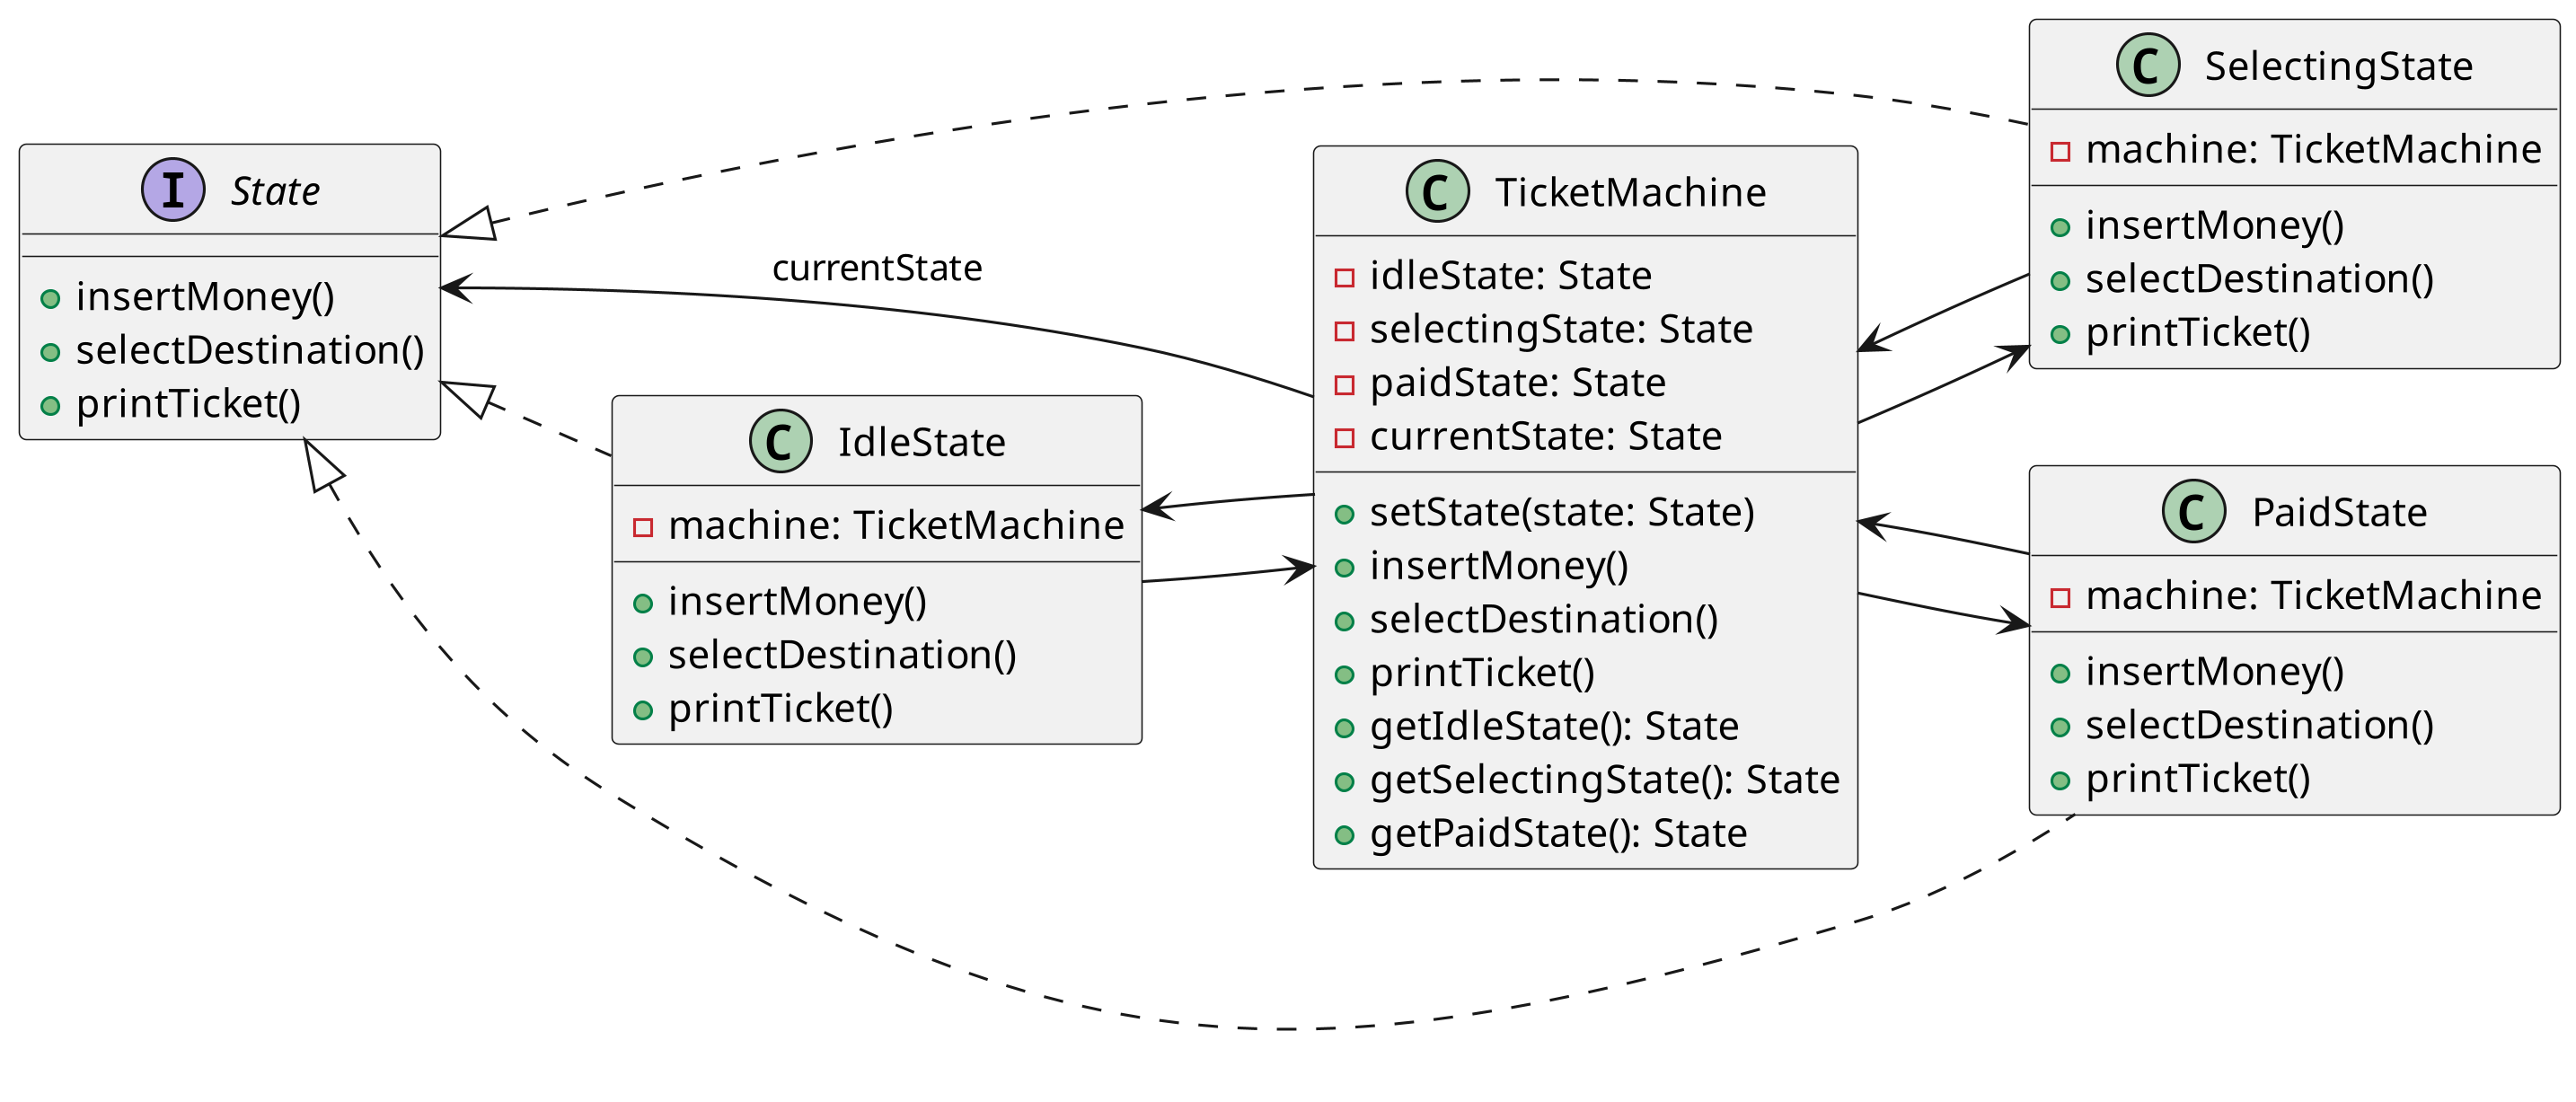
\includegraphics[width=\textwidth]{../figures/out/state.png}
	\caption{Struktur Pola State}
	\label{fig:state}
\end{figure}


\begin{lstlisting}[style=JavaStyle, caption={State Interface}]
	public interface State {
		void insertMoney();
		void selectDestination();
		void printTicket();
	}
\end{lstlisting}

\begin{lstlisting}[style=JavaStyle, caption={ConcreteState: IdleState}]
	public class IdleState implements State {
		private TicketMachine machine;
		
		public IdleState(TicketMachine machine) {
			this.machine = machine;
		}
		
		@Override
		public void insertMoney() {
			System.out.println("Uang diterima.");
			machine.setState(machine.getSelectingState());
		}
		
		@Override
		public void selectDestination() {
			System.out.println("Masukkan uang terlebih dahulu.");
		}
		
		@Override
		public void printTicket() {
			System.out.println("Pilih tujuan terlebih dahulu.");
		}
	}
\end{lstlisting}

\begin{lstlisting}[style=JavaStyle, caption={Context: TicketMachine}]
	public class TicketMachine {
		private State idleState;
		private State selectingState;
		private State paidState;
		
		private State currentState;
		
		public TicketMachine() {
			idleState = new IdleState(this);
			selectingState = new SelectingState(this);
			paidState = new PaidState(this);
			currentState = idleState;
		}
		
		public void setState(State state) {
			this.currentState = state;
		}
		
		public void insertMoney() {
			currentState.insertMoney();
		}
		
		public void selectDestination() {
			currentState.selectDestination();
		}
		
		public void printTicket() {
			currentState.printTicket();
		}
		
		// Getters untuk state
		public State getIdleState() { return idleState; }
		public State getSelectingState() { return selectingState; }
		public State getPaidState() { return paidState; }
	}
\end{lstlisting}

\textbf{Penjelasan:}
\begin{itemize}
	\item \texttt{TicketMachine} bertindak sebagai \texttt{Context} dan menyimpan referensi ke status saat ini.
	\item \texttt{IdleState}, \texttt{SelectingState}, dan \texttt{PaidState} adalah implementasi konkret yang menggambarkan respons mesin berdasarkan status.
	\item Transisi status terjadi melalui pemanggilan \texttt{setState()} di dalam metode \texttt{State} itu sendiri.
\end{itemize}

Pendekatan ini memungkinkan perilaku mesin berubah sesuai dengan status tanpa menggunakan banyak \texttt{if-else} atau \texttt{switch}, menjadikan kode lebih modular, terbaca, dan mudah diperluas.


\section{Chain of Responsibility}
\subsection{Tujuan dan Konteks Penggunaan}

Pola \textit{Chain of Responsibility} merupakan pola desain perilaku yang bertujuan untuk menghindari ketergantungan langsung antara pengirim permintaan dan penerima dengan cara meneruskan permintaan tersebut melalui rantai objek sampai salah satu objek dalam rantai tersebut menangani permintaan tersebut. Setiap objek dalam rantai bertanggung jawab untuk memutuskan apakah akan memproses permintaan atau meneruskannya ke objek berikutnya.

Tujuan utama dari pola ini adalah:
\begin{itemize}
	\item Memisahkan pengirim permintaan dari penerima secara fleksibel.
	\item Menghindari penggunaan banyak pernyataan \texttt{if-else} atau \texttt{switch-case} untuk menangani variasi perilaku.
	\item Memberikan kemungkinan untuk mengubah urutan penanganan permintaan secara dinamis.
\end{itemize}

Struktur dasar dari pola ini terdiri dari:
\begin{itemize}
	\item \textbf{Handler (Interface atau Abstract Class):} Mendefinisikan metode untuk memproses permintaan dan referensi ke handler berikutnya dalam rantai.
	\item \textbf{ConcreteHandler:} Implementasi konkret dari handler yang menangani permintaan tertentu atau meneruskannya ke handler berikutnya.
	\item \textbf{Client:} Pengirim permintaan yang memulai proses dengan handler pertama.
\end{itemize}

Pola ini sangat berguna dalam situasi berikut:
\begin{itemize}
	\item Ketika perlu menangani permintaan yang bisa ditangani oleh lebih dari satu objek, dan objek-objek tersebut dapat dikaitkan secara fleksibel.
	\item Ketika penanganan permintaan tidak perlu diketahui oleh pengirim.
	\item Ketika sistem perlu dikonfigurasi ulang dengan menambah, menghapus, atau mengatur ulang urutan handler tanpa mengubah kode klien.
\end{itemize}

Contoh umum penerapan pola ini antara lain:
\begin{itemize}
	\item Mekanisme validasi berlapis dalam form input atau request HTTP.
	\item Sistem logging dengan beberapa level (debug, info, warning, error).
	\item Sistem approval dalam organisasi (misalnya manajer, direktur, CEO).
	\item Middleware pada framework web modern.
\end{itemize}

Dengan menerapkan pola \textit{Chain of Responsibility}, sistem menjadi lebih fleksibel dan mudah dipelihara karena tanggung jawab dipisahkan dan bisa dikonfigurasi tanpa mengubah logika utama pemrosesan.

\subsection{Contoh Kasus Penggunaan}

Pola \textit{Chain of Responsibility} diterapkan secara luas dalam sistem yang membutuhkan penanganan permintaan secara berlapis atau bertingkat, di mana lebih dari satu objek berpotensi menangani permintaan tersebut. Pola ini memungkinkan implementasi yang fleksibel dan bersifat plug-and-play untuk menambah atau menghapus level penanganan. Berikut adalah beberapa contoh nyata penerapannya:

\textbf{1. Middleware di Framework Web (HTTP Request Handling)} \\
Pada framework seperti Express (Node.js), Spring Boot (Java), atau Phoenix (Elixir), setiap middleware berperan sebagai handler yang menerima permintaan HTTP. Middleware dapat memproses permintaan, memodifikasi konteks, atau meneruskan ke handler berikutnya. Misalnya, middleware autentikasi akan memverifikasi token sebelum permintaan diteruskan ke controller.

\textbf{2. Logger dengan Berbagai Level Prioritas} \\
Sistem logging yang memiliki level seperti \texttt{DEBUG}, \texttt{INFO}, \texttt{WARN}, dan \texttt{ERROR} menggunakan pola ini untuk memproses log berdasarkan level tertentu. Handler untuk level yang lebih tinggi hanya akan merespons pesan log yang relevan dan meneruskan sisanya.

\textbf{3. Sistem Approval Berjenjang} \\
Dalam aplikasi manajemen keuangan atau pengajuan cuti, permintaan disetujui secara bertingkat: supervisor, manajer, hingga direktur. Setiap tingkatan dapat memutuskan untuk menyetujui, menolak, atau meneruskan permintaan ke tingkat berikutnya.

\textbf{4. Validasi Data Formulir} \\
Formulir input pengguna dapat divalidasi menggunakan rantai validator. Misalnya, validasi email, password, dan konfirmasi password masing-masing ditangani oleh validator tersendiri. Jika satu validasi gagal, proses bisa dihentikan atau dilanjutkan tergantung kebijakan.

\textbf{5. Sistem Bantuan Otomatis atau Chatbot} \\
Dalam chatbot, setiap modul (misalnya pertanyaan tentang harga, lokasi, jam operasional) dapat berperan sebagai handler. Jika satu handler tidak bisa menjawab, permintaan diteruskan ke handler lainnya sampai ditemukan jawaban yang sesuai.

\textbf{6. Penanganan Exception atau Error Chaining} \\
Beberapa sistem exception handling menerapkan rantai untuk menangani jenis error yang berbeda. Misalnya, error jaringan, error parsing, dan error database memiliki handler masing-masing dalam satu rantai yang memutuskan apakah akan menangani atau meneruskan.

Penerapan pola ini membantu mengurangi kompleksitas logika bercabang dalam kode (\texttt{if-else}, \texttt{switch-case}) dan memberikan arsitektur yang lebih terbuka untuk ekstensi. Ini menjadikan pola \textit{Chain of Responsibility} sangat ideal untuk sistem dengan proses yang bersifat hierarkis, modular, dan dapat disusun ulang.

\subsection{Kelebihan dan Kekurangan}

Pola \textit{Chain of Responsibility} menawarkan fleksibilitas tinggi dalam mendesain sistem penanganan permintaan yang dapat diproses oleh lebih dari satu objek. Namun seperti pola lainnya, ia juga memiliki batasan yang perlu dipertimbangkan tergantung pada kompleksitas dan kebutuhan sistem.

\textbf{Kelebihan:}
\begin{itemize}
	\item \textbf{Mendukung prinsip open/closed:} Handler baru dapat ditambahkan tanpa memodifikasi struktur yang ada, memungkinkan sistem dikembangkan secara modular.
	\item \textbf{Mengurangi ketergantungan langsung antar komponen:} Objek pengirim permintaan tidak mengetahui objek mana yang akan memprosesnya, sehingga mendorong desain loosely coupled.
	\item \textbf{Memisahkan tanggung jawab secara bersih:} Setiap handler bertanggung jawab hanya terhadap tipe permintaan tertentu, menjaga keterbacaan dan keterurutan kode.
	\item \textbf{Mudah diatur ulang dan diperluas:} Urutan rantai dapat dikonfigurasi secara dinamis berdasarkan kebutuhan konteks eksekusi.
	\item \textbf{Menyederhanakan logika bercabang:} Daripada menggunakan \texttt{if-else} atau \texttt{switch-case} yang panjang, logika dapat disebar ke kelas-kelas handler independen.
\end{itemize}

\textbf{Kekurangan:}
\begin{itemize}
	\item \textbf{Tidak selalu jelas siapa yang menangani permintaan:} Karena permintaan dapat diteruskan sepanjang rantai, sulit untuk memastikan secara eksplisit siapa yang akan mengeksekusi aksi.
	\item \textbf{Debugging lebih rumit:} Jejak eksekusi bisa menjadi tidak linear dan menyulitkan proses pelacakan masalah, terutama pada rantai yang panjang.
	\item \textbf{Overhead performa:} Jika permintaan harus melewati banyak handler sebelum ditangani, ini dapat menyebabkan penurunan efisiensi.
	\item \textbf{Risiko handler saling bergantung:} Jika tidak dirancang dengan benar, handler bisa menjadi terlalu sadar akan urutan rantai atau handler lain, yang justru mengurangi fleksibilitas.
	\item \textbf{Kesalahan logika dalam penerusan:} Bila handler lupa meneruskan permintaan (jika tidak diproses), permintaan bisa berhenti tanpa hasil, terutama jika tidak ada fallback handler.
\end{itemize}

Secara keseluruhan, pola \textit{Chain of Responsibility} sangat bermanfaat untuk sistem yang perlu memproses permintaan secara berlapis. Namun, ia perlu diterapkan dengan struktur yang jelas dan dokumentasi yang baik agar tetap dapat dipelihara dan dipahami seiring berkembangnya sistem.


\subsection{Implementasi dalam Java}

Implementasi pola \textit{Chain of Responsibility} dalam Java umumnya dilakukan dengan mendefinisikan antarmuka atau kelas abstrak \texttt{Handler} yang menyatakan kontrak penanganan permintaan dan referensi ke handler berikutnya dalam rantai. Setiap \texttt{ConcreteHandler} kemudian mengimplementasikan logika spesifik untuk memproses atau meneruskan permintaan.

Struktur umum implementasinya terdiri dari:

\begin{itemize}
	\item \textbf{Handler (Interface / Abstract Class):} Mendefinisikan metode untuk menangani permintaan dan menetapkan handler selanjutnya (next handler).
	\item \textbf{ConcreteHandler:} Kelas-kelas konkret yang memeriksa apakah mereka bisa menangani permintaan, jika tidak maka diteruskan ke handler berikutnya.
	\item \textbf{Client:} Menginisialisasi rantai handler dan mengirimkan permintaan awal.
\end{itemize}


\begin{figure}[h]
	\centering
	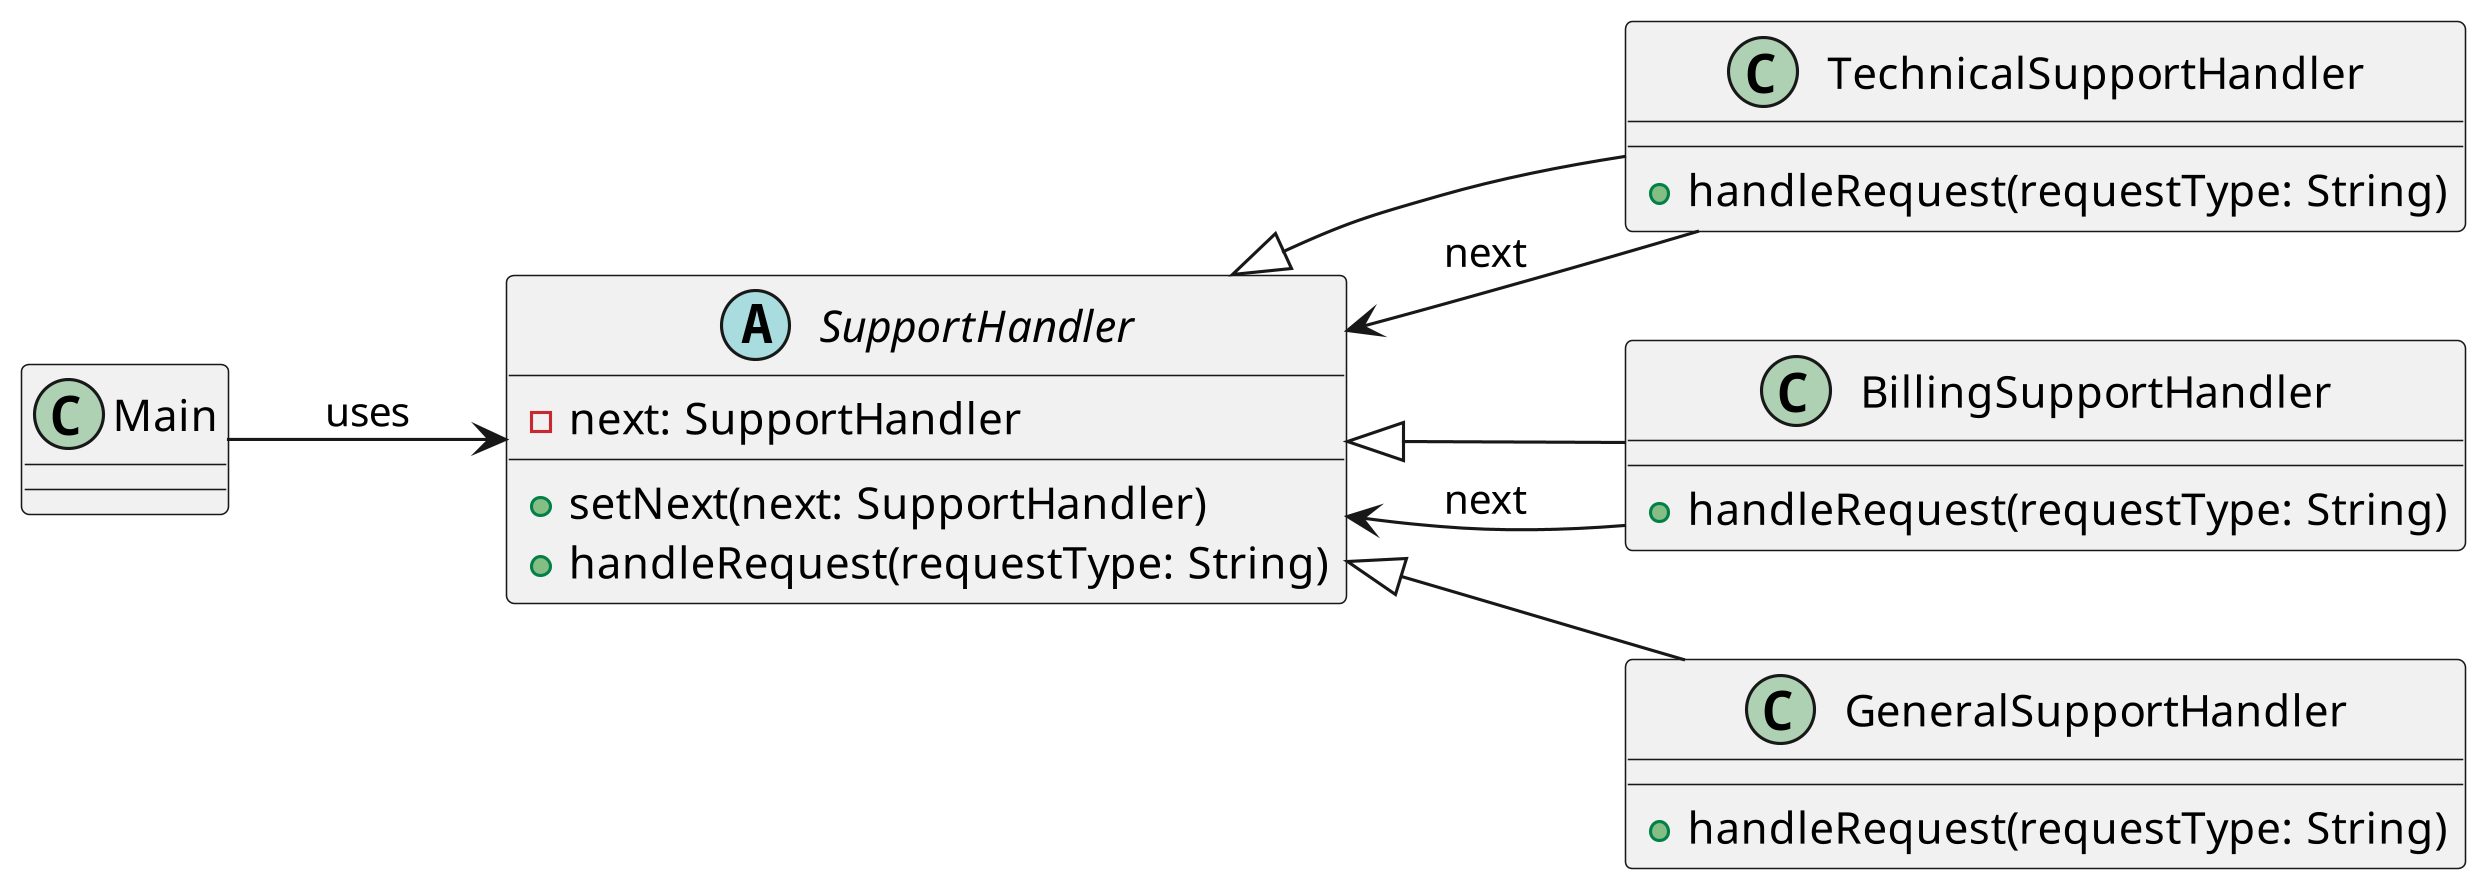
\includegraphics[width=\textwidth]{../figures/out/chain_of_responsibility.png}
	\caption{Struktur Pola State}
	\label{fig:chain_of_responsibility}
\end{figure}

Contoh implementasi (Gambar~\ref{fig:chain_of_responsibility}) berikut menunjukkan sistem validasi permintaan dukungan pelanggan berdasarkan kategori permintaan:



\begin{lstlisting}[style=JavaStyle, caption={Antarmuka Handler}]
	public abstract class SupportHandler {
		protected SupportHandler next;
		
		public void setNext(SupportHandler next) {
			this.next = next;
		}
		
		public abstract void handleRequest(String requestType);
	}
\end{lstlisting}

\begin{lstlisting}[style=JavaStyle, caption={Handler untuk Permintaan Teknis}]
	public class TechnicalSupportHandler extends SupportHandler {
		@Override
		public void handleRequest(String requestType) {
			if ("Technical".equalsIgnoreCase(requestType)) {
				System.out.println("Ditangani oleh tim teknis.");
			} else if (next != null) {
				next.handleRequest(requestType);
			}
		}
	}
\end{lstlisting}

\begin{lstlisting}[style=JavaStyle, caption={Handler untuk Permintaan Penagihan}]
	public class BillingSupportHandler extends SupportHandler {
		@Override
		public void handleRequest(String requestType) {
			if ("Billing".equalsIgnoreCase(requestType)) {
				System.out.println("Ditangani oleh tim penagihan.");
			} else if (next != null) {
				next.handleRequest(requestType);
			}
		}
	}
\end{lstlisting}

\begin{lstlisting}[style=JavaStyle, caption={Handler Default}]
	public class GeneralSupportHandler extends SupportHandler {
		@Override
		public void handleRequest(String requestType) {
			System.out.println("Ditangani oleh tim umum.");
		}
	}
\end{lstlisting}

\begin{lstlisting}[style=JavaStyle, caption={Client: Membentuk Rantai dan Mengirim Permintaan}]
	public class Main {
		public static void main(String[] args) {
			SupportHandler tech = new TechnicalSupportHandler();
			SupportHandler billing = new BillingSupportHandler();
			SupportHandler general = new GeneralSupportHandler();
			
			tech.setNext(billing);
			billing.setNext(general);
			
			tech.handleRequest("Billing");
			tech.handleRequest("Technical");
			tech.handleRequest("Feedback");
		}
	}
\end{lstlisting}

\textbf{Penjelasan:}

\begin{itemize}
	\item \texttt{SupportHandler} adalah kelas abstrak yang mendefinisikan rantai dan metode \texttt{handleRequest()}.
	\item Setiap \texttt{ConcreteHandler} menangani permintaan sesuai tipe tertentu.
	\item Jika handler tidak cocok, ia meneruskan permintaan ke handler berikutnya.
	\item Rantai dapat dikonfigurasi ulang di \texttt{Client}, memberikan fleksibilitas dalam pengaturan urutan dan logika pemrosesan.
\end{itemize}

Pola ini sangat cocok digunakan dalam sistem seperti filter permintaan HTTP, middleware pipeline, validasi bertingkat, atau sistem bantuan pengguna dengan tingkatan dukungan berbeda.



\section{Template Method}
\subsection{Tujuan dan Konteks Penggunaan}

Pola \textit{Template Method} adalah pola desain perilaku yang digunakan untuk mendefinisikan kerangka (template) dari suatu algoritma di dalam kelas induk (superclass), sambil memungkinkan subclass untuk mengisi atau mengubah bagian-bagian tertentu dari algoritma tersebut tanpa mengubah struktur keseluruhan. Pola ini mengikuti prinsip \textit{Hollywood Principle}: "Don't call us, we'll call you", artinya kelas induk memegang kendali alur proses dan hanya memanggil metode-metode yang didefinisikan ulang oleh kelas turunan saat diperlukan.

Tujuan utama dari pola \textit{Template Method} adalah:

\begin{itemize}
	\item \textbf{Mendefinisikan alur algoritma secara konsisten di satu tempat (superclass)} agar tidak duplikatif di setiap implementasi.
	\item \textbf{Memungkinkan variasi perilaku di tahap-tahap tertentu} tanpa mengubah struktur umum proses.
	\item \textbf{Memisahkan logika yang tetap dan yang dapat berubah} dalam suatu proses, sehingga lebih mudah dipelihara dan dikembangkan.
\end{itemize}

Pola ini sering digunakan ketika terdapat sejumlah langkah umum yang selalu dilakukan dalam urutan tertentu, tetapi rincian dari satu atau beberapa langkah bisa berbeda tergantung konteks. Subclass dapat mengimplementasikan langkah-langkah ini melalui metode abstrak atau metode hook yang tersedia.

Struktur utama pola ini mencakup:

\begin{itemize}
	\item \textbf{AbstractClass:} Kelas induk yang mendefinisikan template method dan beberapa metode abstrak (atau hook) yang bisa ditimpa.
	\item \textbf{ConcreteClass:} Kelas turunan yang menyediakan implementasi spesifik untuk langkah-langkah yang didefinisikan dalam template.
\end{itemize}

Pola \textit{Template Method} umum digunakan dalam sistem yang memiliki pola proses tetap, seperti proses otentikasi, pipeline pemrosesan data, sistem rendering, dan berbagai jenis workflow atau proses batch. Dengan pendekatan ini, pengembang dapat mempertahankan kontrol atas urutan langkah sambil memberikan fleksibilitas pada detail implementasinya.

\subsection{Contoh Kasus Penggunaan}

Pola \textit{Template Method} sangat berguna dalam sistem yang memiliki struktur proses atau algoritma yang tetap, tetapi mengizinkan sebagian langkah diubah oleh subclass. Berikut adalah beberapa contoh nyata penerapannya:

\textbf{1. Proses Login dan Autentikasi} \\
Dalam aplikasi web atau desktop, proses login biasanya terdiri dari langkah-langkah tetap: mengambil kredensial, memvalidasi input, mengecek akun di database, dan memberikan akses. Langkah-langkah ini bisa didefinisikan sebagai template dalam kelas abstrak, sementara mekanisme autentikasi (misalnya dengan username/password, OTP, atau OAuth) diimplementasikan oleh subclass.

\textbf{2. Sistem Proses Dokumen (Document Workflow)} \\
Dalam aplikasi pengelolaan dokumen (misalnya approval sistem), urutan proses seperti membaca dokumen, memverifikasi format, memproses isi, dan menyimpan hasil bisa dijadikan template. Setiap jenis dokumen (PDF, Word, XML) dapat menjadi subclass yang mengisi detail spesifik proses pembacaan dan pemrosesan.

\textbf{3. Game Engine: Siklus Game Loop} \\
Game loop sering kali memiliki urutan tetap: update input, update state, render ke layar. Template method digunakan untuk menetapkan struktur ini di kelas abstrak, sedangkan tiap game atau level mengisi detail langkah-langkah tersebut (misalnya bagaimana input diproses atau bagaimana render dilakukan).

\textbf{4. Laporan dan Ekspor Data} \\
Aplikasi bisnis yang menghasilkan laporan dalam berbagai format (Excel, PDF, CSV) dapat menggunakan template method untuk mengatur alur ekspor: menyiapkan data, memformat, dan menyimpan file. Format laporan diatur oleh subclass masing-masing.

\textbf{5. Unit Test Framework} \\
Dalam framework pengujian (seperti JUnit), kerangka pengujian terdiri dari langkah-langkah seperti setup, eksekusi tes, dan teardown. Framework menyediakan template method, sementara pengguna menyediakan subclass yang mengimplementasikan test case.

\textbf{6. Sistem Pembayaran atau Transaksi} \\
Proses pembayaran pada umumnya mengikuti alur tetap: validasi, otorisasi, eksekusi transaksi, dan pencatatan. Namun, implementasi detail untuk metode pembayaran berbeda (kartu kredit, e-wallet, transfer) dapat diatur oleh subclass menggunakan pola \textit{Template Method}.

Melalui pola ini, pengembang dapat menjaga alur logika tetap konsisten sembari mengizinkan variasi dalam pelaksanaannya. Hal ini menjadikan sistem lebih mudah dikembangkan, diuji, dan dipelihara karena struktur algoritma utama hanya ditulis sekali di superclass.

\subsection{Kelebihan dan Kekurangan}

Pola \textit{Template Method} memiliki sejumlah keunggulan yang membuatnya sangat berguna dalam situasi di mana terdapat algoritma dengan struktur tetap, namun sebagian langkahnya dapat divariasikan. Namun demikian, penerapannya juga memiliki keterbatasan yang harus diperhatikan dalam desain perangkat lunak.

\textbf{Kelebihan:}
\begin{itemize}
	\item \textbf{Mendukung reuse dan standar proses:} Pola ini memungkinkan pengembang untuk mendefinisikan alur algoritma sekali di superclass dan mewariskannya ke subclass, sehingga mencegah duplikasi dan memastikan konsistensi proses.
	
	\item \textbf{Menerapkan prinsip Hollywood:} Subclass hanya menyediakan detail pelaksanaan langkah, sementara struktur utama tetap dikendalikan oleh superclass (prinsip "Don't call us, we'll call you").
	
	\item \textbf{Mempermudah pemeliharaan kode:} Ketika struktur proses berubah, hanya superclass yang perlu diubah. Subclass tetap berfungsi selama antarmuka metode tetap konsisten.
	
	\item \textbf{Cocok untuk framework dan library:} Pola ini mendukung pengembangan framework yang dapat diperluas oleh pengguna tanpa mengubah struktur dasar framework tersebut.
	
	\item \textbf{Mendukung perluasan tanpa modifikasi:} Langkah-langkah algoritma dapat ditambah atau disesuaikan melalui subclass baru, sesuai dengan prinsip Open/Closed.
\end{itemize}

\textbf{Kekurangan:}
\begin{itemize}
	\item \textbf{Keterikatan antar kelas meningkat:} Subclass sangat bergantung pada struktur superclass. Jika struktur superclass berubah, semua subclass bisa terdampak dan memerlukan penyesuaian.
	
	\item \textbf{Sulit dipahami jika terlalu dalam:} Hierarki kelas yang terlalu dalam atau kompleks bisa membuat alur eksekusi sulit ditelusuri, terutama saat debugging.
	
	\item \textbf{Keterbatasan fleksibilitas runtime:} Karena subclass harus ditentukan secara eksplisit pada saat kompilasi, pola ini kurang fleksibel jika dibandingkan dengan pola seperti \textit{Strategy} yang mendukung pertukaran perilaku saat runtime.
	
	\item \textbf{Resiko implementasi kosong:} Dalam beberapa kasus, subclass tidak perlu mengimplementasikan semua langkah, sehingga menghasilkan metode kosong yang bisa menurunkan kualitas desain.
	
	\item \textbf{Kurang cocok untuk proses sangat dinamis:} Jika setiap langkah dalam proses sering berubah atau sangat bergantung pada konfigurasi eksternal, pendekatan berbasis komposisi lebih tepat daripada inheritance.
\end{itemize}

Secara keseluruhan, pola \textit{Template Method} sangat efektif digunakan dalam sistem yang memerlukan struktur proses tetap namun fleksibel dalam pelaksanaan langkah-langkahnya. Penggunaan pola ini harus diseimbangkan dengan kompleksitas pewarisan dan kebutuhan fleksibilitas runtime.

\subsection{Implementasi dalam Java}

Implementasi pola \textit{Template Method} dalam Java dilakukan dengan cara mendefinisikan kerangka algoritma dalam kelas abstrak (abstract class) dan membiarkan subclass mengimplementasikan langkah-langkah tertentu dari algoritma tersebut. Kelas abstrak menyediakan satu metode utama (template method) yang berisi urutan langkah-langkah tetap, sementara beberapa langkah tersebut dideklarasikan sebagai metode abstrak atau metode \textit{hook} (opsional untuk di-override).

Struktur umumnya terdiri dari:
\begin{itemize}
	\item \textbf{AbstractClass:} Kelas abstrak yang berisi \texttt{templateMethod()} sebagai kerangka alur dan mendefinisikan metode abstrak untuk langkah-langkah yang perlu disesuaikan oleh subclass.
	\item \textbf{ConcreteClass:} Kelas konkret yang mengimplementasikan metode-metode abstrak dan (opsional) override metode \textit{hook}.
\end{itemize}


\begin{figure}[h]
	\centering
	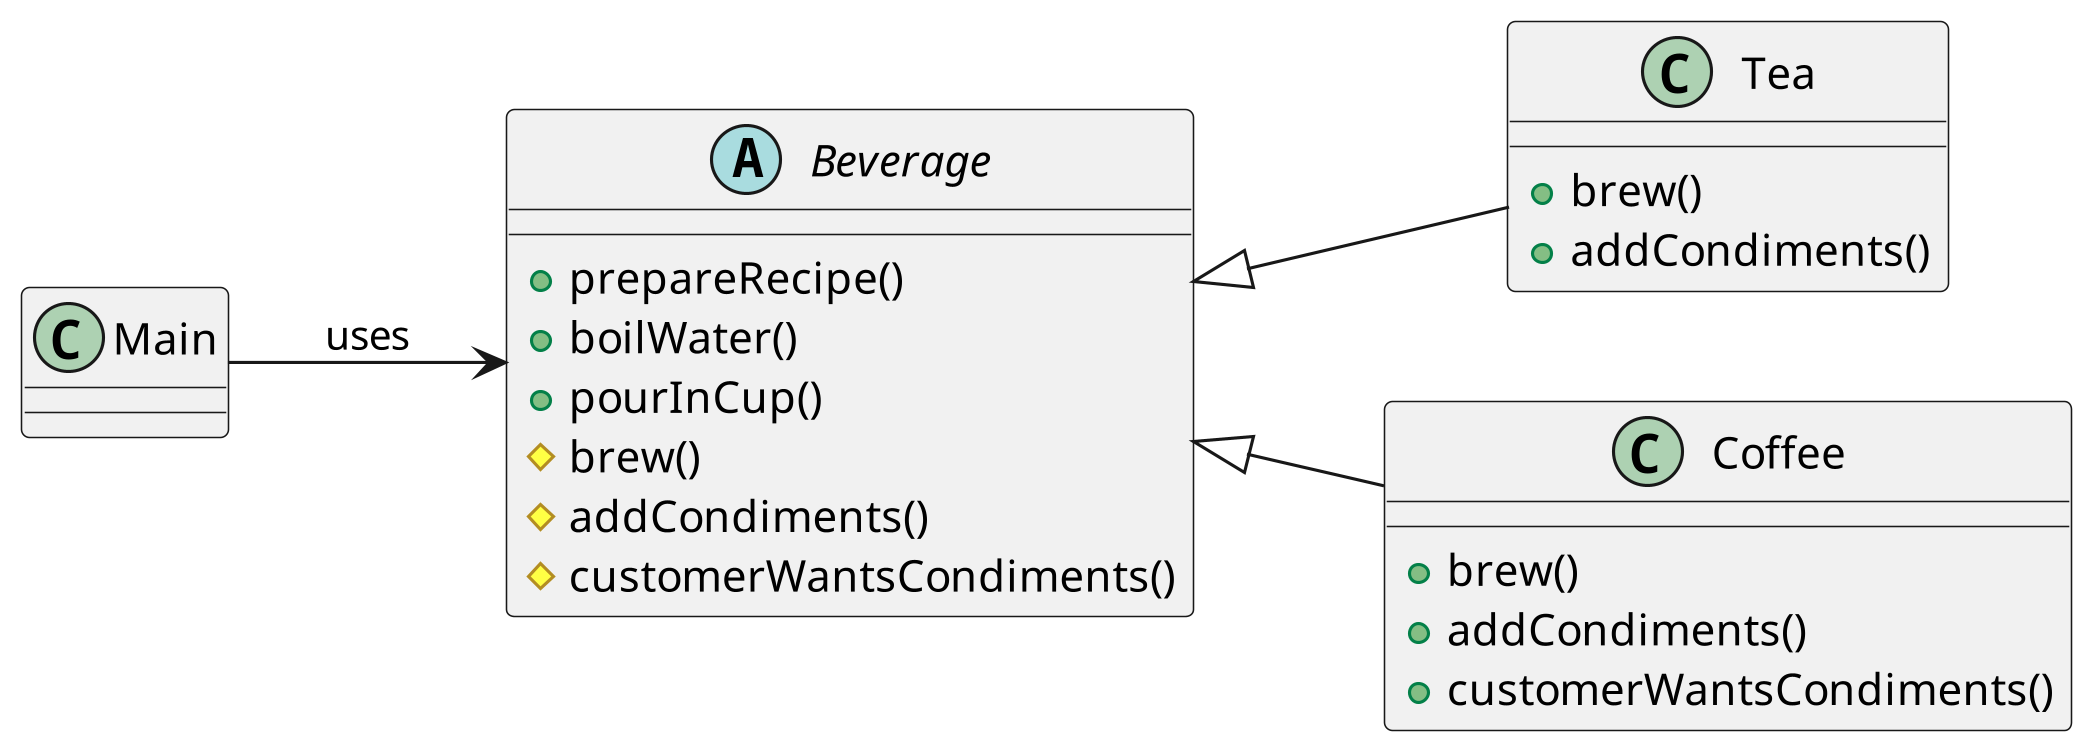
\includegraphics[width=\textwidth]{../figures/out/template_method.png}
	\caption{Struktur Pola State}
	\label{fig:template_method}
\end{figure}


Contoh berikut menggambarkan proses pembuatan minuman (misalnya teh dan kopi) yang memiliki langkah tetap: mendidihkan air, menyeduh bahan, menuang ke cangkir, dan (opsional) menambahkan tambahan (Gambar\ref{fig:template_method}).

\begin{lstlisting}[style=JavaStyle, caption={Kelas Abstrak dengan Template Method}]
	public abstract class Beverage {
		public final void prepareRecipe() {
			boilWater();
			brew();
			pourInCup();
			if (customerWantsCondiments()) {
				addCondiments();
			}
		}
		
		protected void boilWater() {
			System.out.println("Boiling water");
		}
		
		protected void pourInCup() {
			System.out.println("Pouring into cup");
		}
		
		protected abstract void brew();
		protected abstract void addCondiments();
		
		// Hook method
		protected boolean customerWantsCondiments() {
			return true;
		}
	}
\end{lstlisting}

\begin{lstlisting}[style=JavaStyle, caption={Subclass untuk Teh}]
	public class Tea extends Beverage {
		@Override
		protected void brew() {
			System.out.println("Steeping the tea");
		}
		
		@Override
		protected void addCondiments() {
			System.out.println("Adding lemon");
		}
	}
\end{lstlisting}

\begin{lstlisting}[style=JavaStyle, caption={Subclass untuk Kopi}]
	public class Coffee extends Beverage {
		@Override
		protected void brew() {
			System.out.println("Dripping coffee through filter");
		}
		
		@Override
		protected void addCondiments() {
			System.out.println("Adding sugar and milk");
		}
		
		@Override
		protected boolean customerWantsCondiments() {
			return false; // tanpa tambahan
		}
	}
\end{lstlisting}

\begin{lstlisting}[style=JavaStyle, caption={Client Code}]
	public class Main {
		public static void main(String[] args) {
			Beverage tea = new Tea();
			tea.prepareRecipe();
			
			System.out.println();
			
			Beverage coffee = new Coffee();
			coffee.prepareRecipe();
		}
	}
\end{lstlisting}

Penjelasan:
\begin{itemize}
	\item \texttt{prepareRecipe()} adalah metode template yang tidak boleh diubah oleh subclass.
	\item Metode \texttt{brew()} dan \texttt{addCondiments()} bersifat abstrak dan wajib diimplementasikan di subclass.
	\item \texttt{customerWantsCondiments()} adalah metode \textit{hook} yang dapat dioverride untuk mengatur perilaku opsional.
\end{itemize}

Pola ini ideal ketika proses utama bersifat tetap namun beberapa langkah dapat bervariasi tergantung implementasi. Pendekatan ini mendukung reuse, keterbacaan, dan konsistensi proses dalam hierarki kelas.

\section{Kesimpulan}

Pola-pola desain perilaku lanjutan—\textit{Mediator}, \textit{State}, \textit{Chain of Responsibility}, dan \textit{Template Method} -- menawarkan pendekatan struktural yang kuat untuk mengelola interaksi, perubahan status, alur tanggung jawab, dan urutan eksekusi dalam sistem perangkat lunak. Pola \textit{Mediator} memusatkan komunikasi antar objek dalam satu komponen, mengurangi kompleksitas dan ketergantungan langsung antar komponen. Pola \textit{State} memungkinkan objek mengubah perilakunya sesuai dengan kondisi internal, mendukung sistem yang membutuhkan pengelolaan transisi status secara fleksibel. Sementara itu, \textit{Chain of Responsibility} menyusun objek pemroses dalam rantai dinamis, memungkinkan penanganan permintaan secara fleksibel tanpa mengetahui handler mana yang akan menangani. 

Adapun \textit{Template Method} memberikan struktur algoritma tetap sekaligus membiarkan bagian-bagian tertentu disesuaikan oleh subclass, menjadikannya cocok untuk sistem dengan pola langkah yang konsisten. Dengan menerapkan pola-pola ini secara tepat, pengembang dapat membangun sistem yang modular, mudah diuji, dan siap diperluas. Pemilihan pola perlu mempertimbangkan konteks kebutuhan, tingkat fleksibilitas, serta konsistensi alur logika aplikasi yang diinginkan.

